\documentclass{article}

\usepackage[margin=1.5cm]{geometry}
\usepackage{parskip}
\usepackage{graphicx}
\usepackage{multicol}
\usepackage[ruled]{algorithm2e}
\usepackage{amsmath}
\usepackage{subcaption}

\title{MAT004 - Example Coursework}
\author{Geraint Palmer - c1016865}
\date{}

\begin{document}

\maketitle

\section{Introduction \& Problem}
Josie's shed is a chain garden stores based in France. They would like to start an radio advertising campaign that will reach the following 30 cities in France:

\begin{multicols}{5}
\begin{itemize}
  \setlength\itemsep{-0.5em}
  \item Amiens
  \item Avignon
  \item Biarritz
  \item Bordeaux
  \item Brest
  \item Caen
  \item Calais
  \item Dijon
  \item Grenoble
  \item La Rochelle
  \item Le Havre
  \item Le Mans
  \item Lille
  \item Limoges
  \item Lyon
  \item Marseilles
  \item Montpellier
  \item Nancy
  \item Nantes
  \item Nice
  \item Orleans
  \item Paris
  \item Perpignon
  \item Poitiers
  \item Reims
  \item Rennes
  \item Rouen
  \item Stranbourg
  \item Toulon
  \item Toulouse
\end{itemize}
\end{multicols}

Each city has it's own radio station whose broadcast can reach different distances, and so reach different cities, according to an adjacency matrix. Figure~\ref{fig:adjacency} shows the reach of the broadcast in different cities, with an edge connecting cities if they can hear each others' broadcasts.
Josie's Shed would like to know the minimum number of cities they need to broadcast from in order to reach all thirty French cities. This is an example of the \textit{dominating set problem}.

\section{Methodology}
A simple heuristic neighbourhood search algorithm will be used.
Here neighbourhood operator is selecting a random set of cities.
It is evaluated by checking if that set is a dominating set, if so, then the cost of that set is the size of the set. Otherwise the cost of that set is 30, the number of cities, as it would be better to choose every city (and so reach every city) than to choose a non-dominating set.
If the cost of that set is smaller than the previous best solution, then that is labelled as the best solution.
This is repeated a number of times. This algorithm is shown in Figure~\ref{fig:algorithm}.

\begin{algorithm}
\KwData{$\mathbf{A}$ an adjacency matrix; $n$ the number of iterations}
\KwResult{$\mathbf{s}_\star$, a minimal dominating set.}
$m \gets$ size of $\mathbf{A}$\;
$i \gets 0$\;
$c \gets \operatorname{rank}(\mathbf{A})$\;
$b \gets m$\;
Let $\mathbf{s}_\star$ be a vector of $m$ ones.\;
\While{$i \leq n $}{
  Let $\mathbf{s}$ be a random vector containing $c$ ones and $m-c$ zeros\;
  $\mathbf{r} \gets \mathbf{A}\mathbf{s}$\;
  \If{$0 \notin \mathbf{r}$}{
    $b \gets m$\;
    $\mathbf{s}_\star \gets \mathbf{s}$\;
    $c \gets c - 1$\;
  }
}
\caption{A neighbourhood search algorithm.}
\label{fig:algorithm}
\end{algorithm}

Here $\mathbf{A}$ is the adjacency matrix, $n$ is the number of iterations, $m$ is the number of cities, $c$ is the current number of cities to try to find a dominating set, $i$ is the current iteration, $b$ is the current best cost, and $\mathbf{s}_\star$ is the current best solution.

Note that the vector $\mathbf{r} = \mathbf{A}\mathbf{s}$ is a vector giving, for each city, the number of cities in $\mathbf{s}$ they see. Therefore if this contains a $0$ then there is at least one city that is not seen by the cities of $\mathbf{s}$, and so if it doesn't contain a $0$ then this is a dominating set.

Note also that we begin with $c = \operatorname{rank}(\mathbf{A})$. The rank of a matrix is the number of linearly dependent rows, and so in an adjacency matrix, whose elements are either 0 or 1, it is the number of identical rows. If two rows are identical, then the two corresponding cities see the same cities, and should never be chosen together. Therefore we know we can find a solution of size $\operatorname{rank}(\mathbf{A})$.


\section{Results}
When run for 5000 iterations we get a solution containing just 7 cities in the dominating set. This is shown in Figure~\ref{fig:solution}. The chosen cities are: Avignon, Bordeaux, Limoges, Nancy, Nice, Rennes, and Rouen.

The number of iterations, 5000, was chosen arbitrarily. The higher the number of iterations, the better the solution, as we are more likely to randomly find the dominating sets. Figure~\ref{fig:overtime} shows the relationship between iterations and number of cities in the dominating set. We see that very quickly a good solution of 10 cities is found, but it takes a very large number of iterations before any better solutions are found.

\begin{figure}
\centering
\begin{subfigure}{0.45\textwidth}
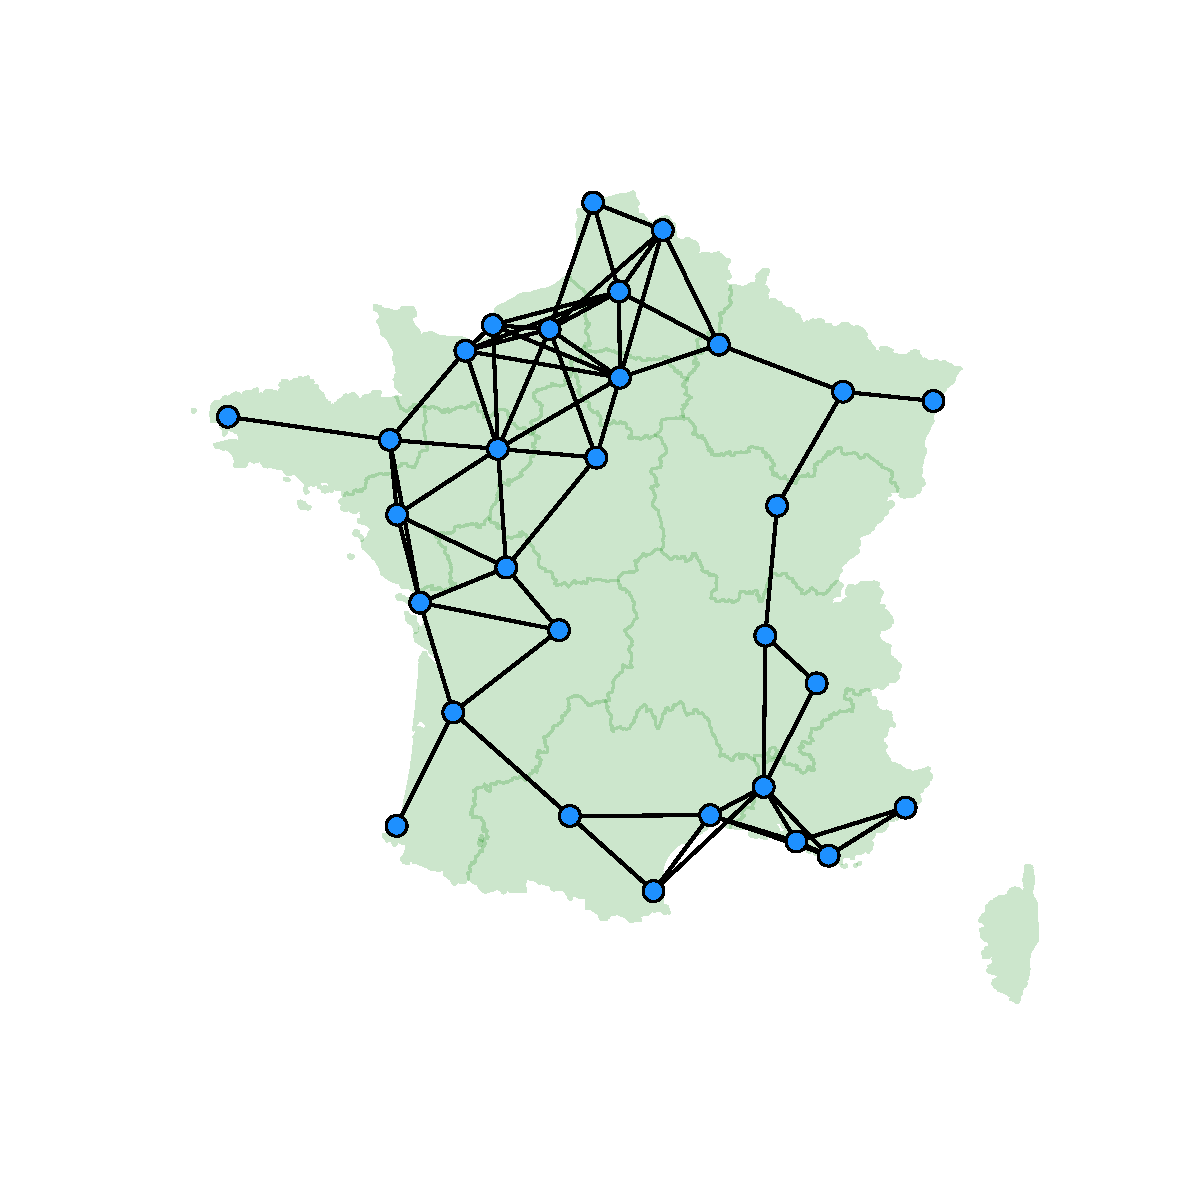
\includegraphics[width=\textwidth]{adjacency}
\caption{Map of cities who can mutually hear each others' radio broadcasts.}
\label{fig:adjacency}
\end{subfigure}
\hfill
\begin{subfigure}{0.45\textwidth}
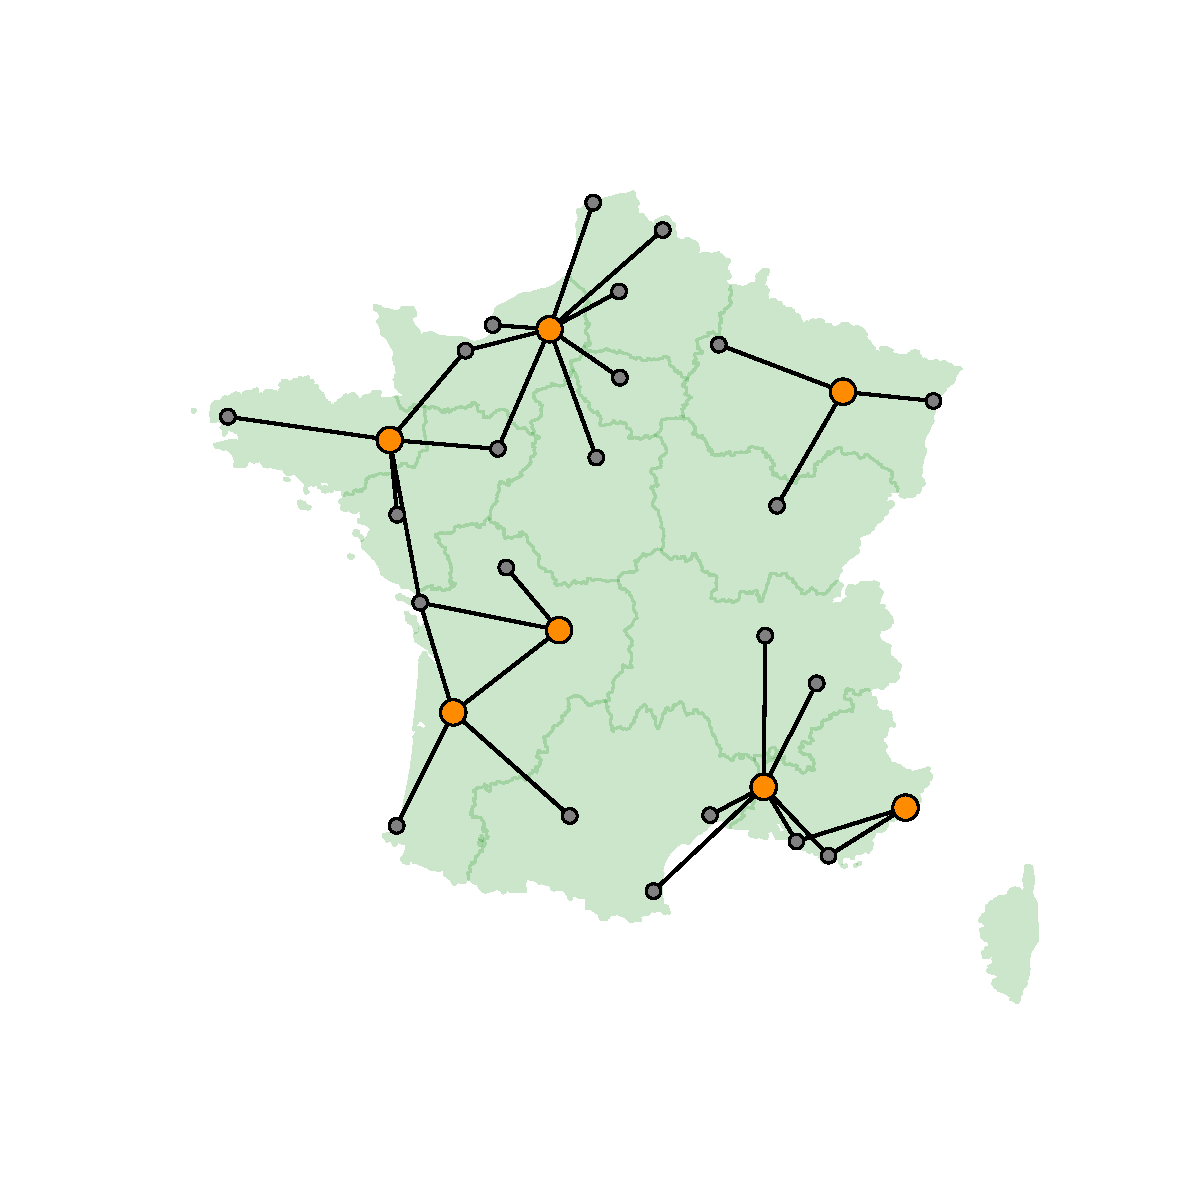
\includegraphics[width=\textwidth]{solution}
\caption{Map of solution with 7 cities in the dominating set (orange).}
\label{fig:solution}
\end{subfigure}
\end{figure}

\begin{figure}
\centering
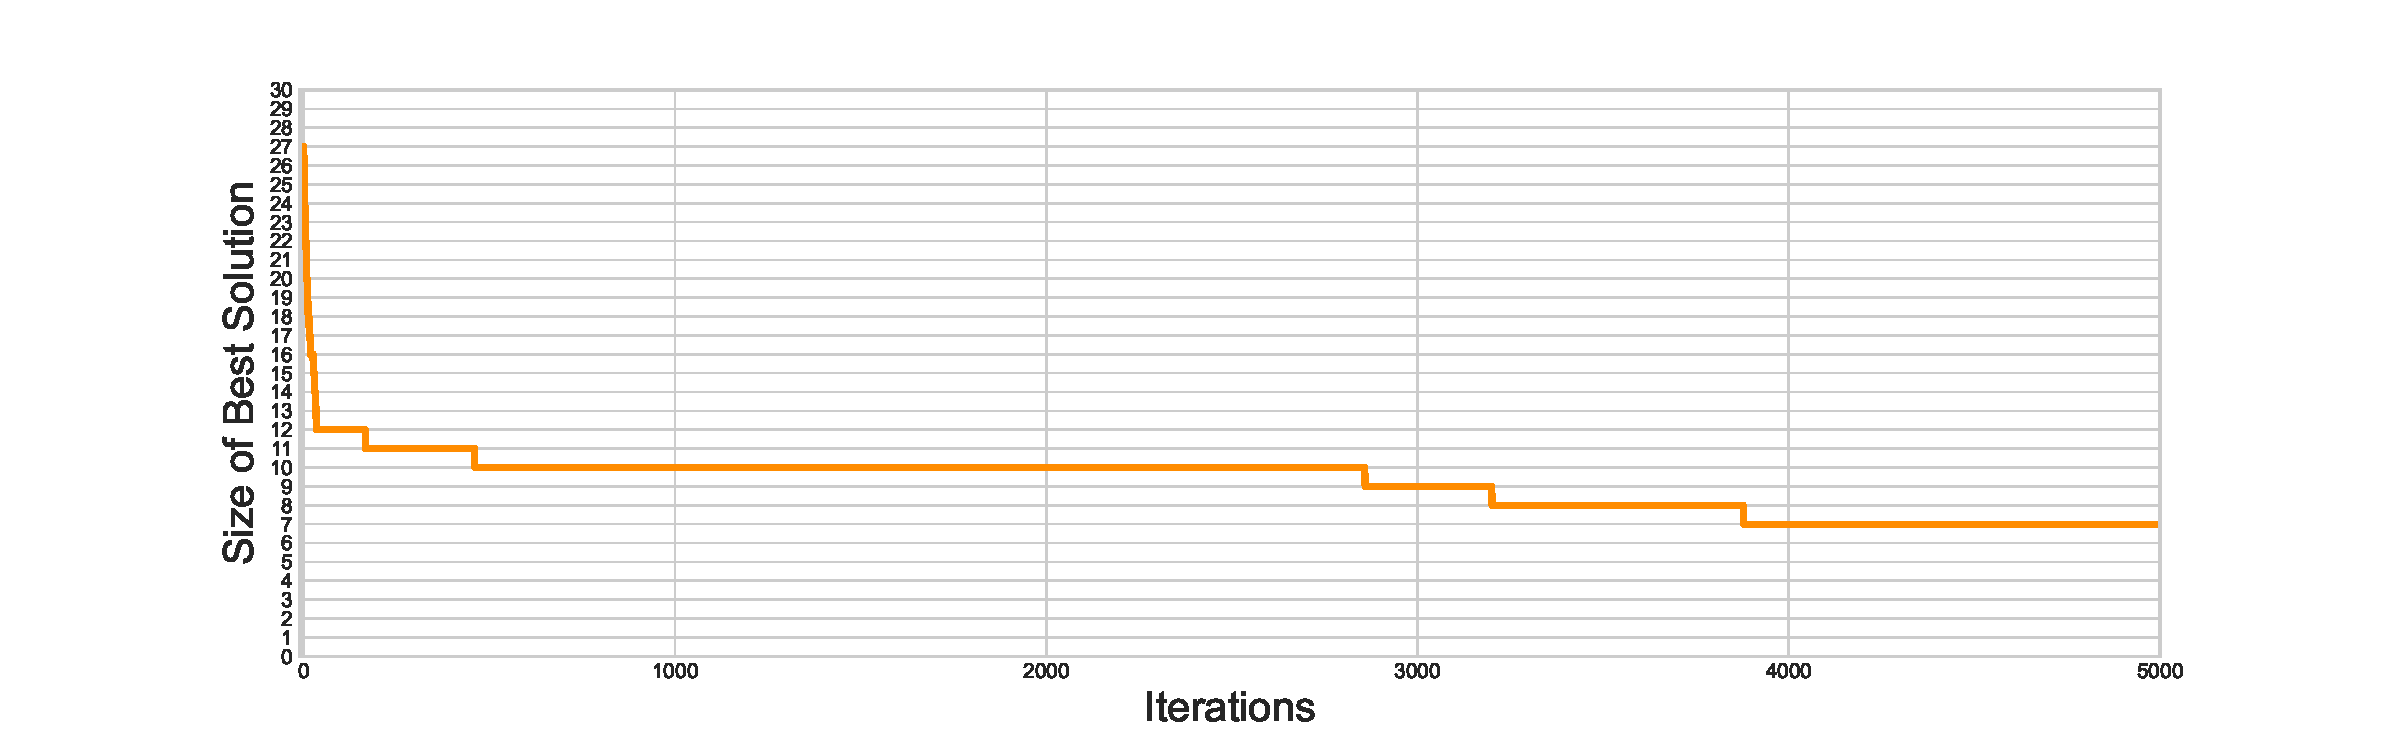
\includegraphics[width=0.75\textwidth]{overtime}
\caption{Plot of the best solution $b$ over time.}
\label{fig:overtime}
\end{figure}

\end{document}